\section{Systemarchitektur und Rahmenbedingungen}
Die Konzeption eines produktiv einsetzbaren Empfehlungssystems für die SV-Gruppe erfordert eine Architektur, die klar definierten Rahmenbedingungen genügt. Aus dem Anwendungsfall lassen sich nicht-funktionale Anforderungen ableiten, die die technische Ausgestaltung leiten.
\label{sec:nfr}

Für den initialen Proof-of-Concept wurden drei erfolgskritische \ac{NFR}s identifiziert:
Erstens muss das System niedrige Antwortzeiten unter Last gewährleisten. Als konkretes \ac{SLO} wird eine End-to-End-Latenz im 95. Perzentil von unter 2000 Millisekunden angestrebt.
Zweitens ist eine horizontale Skalierbarkeit erforderlich, um auf wachsende Nutzerzahlen und Datenmengen im dynamischen Umfeld eines Nachrichtenportals reagieren zu können.
Drittens ist eine einfache Integrierbarkeit sicherzustellen; hierzu wird eine standardisierte REST-API bereitgestellt, die die Einbindung in bestehende Redaktions- und IT-Workflows vereinfacht.
\begin{figure}[H]
    \centering
    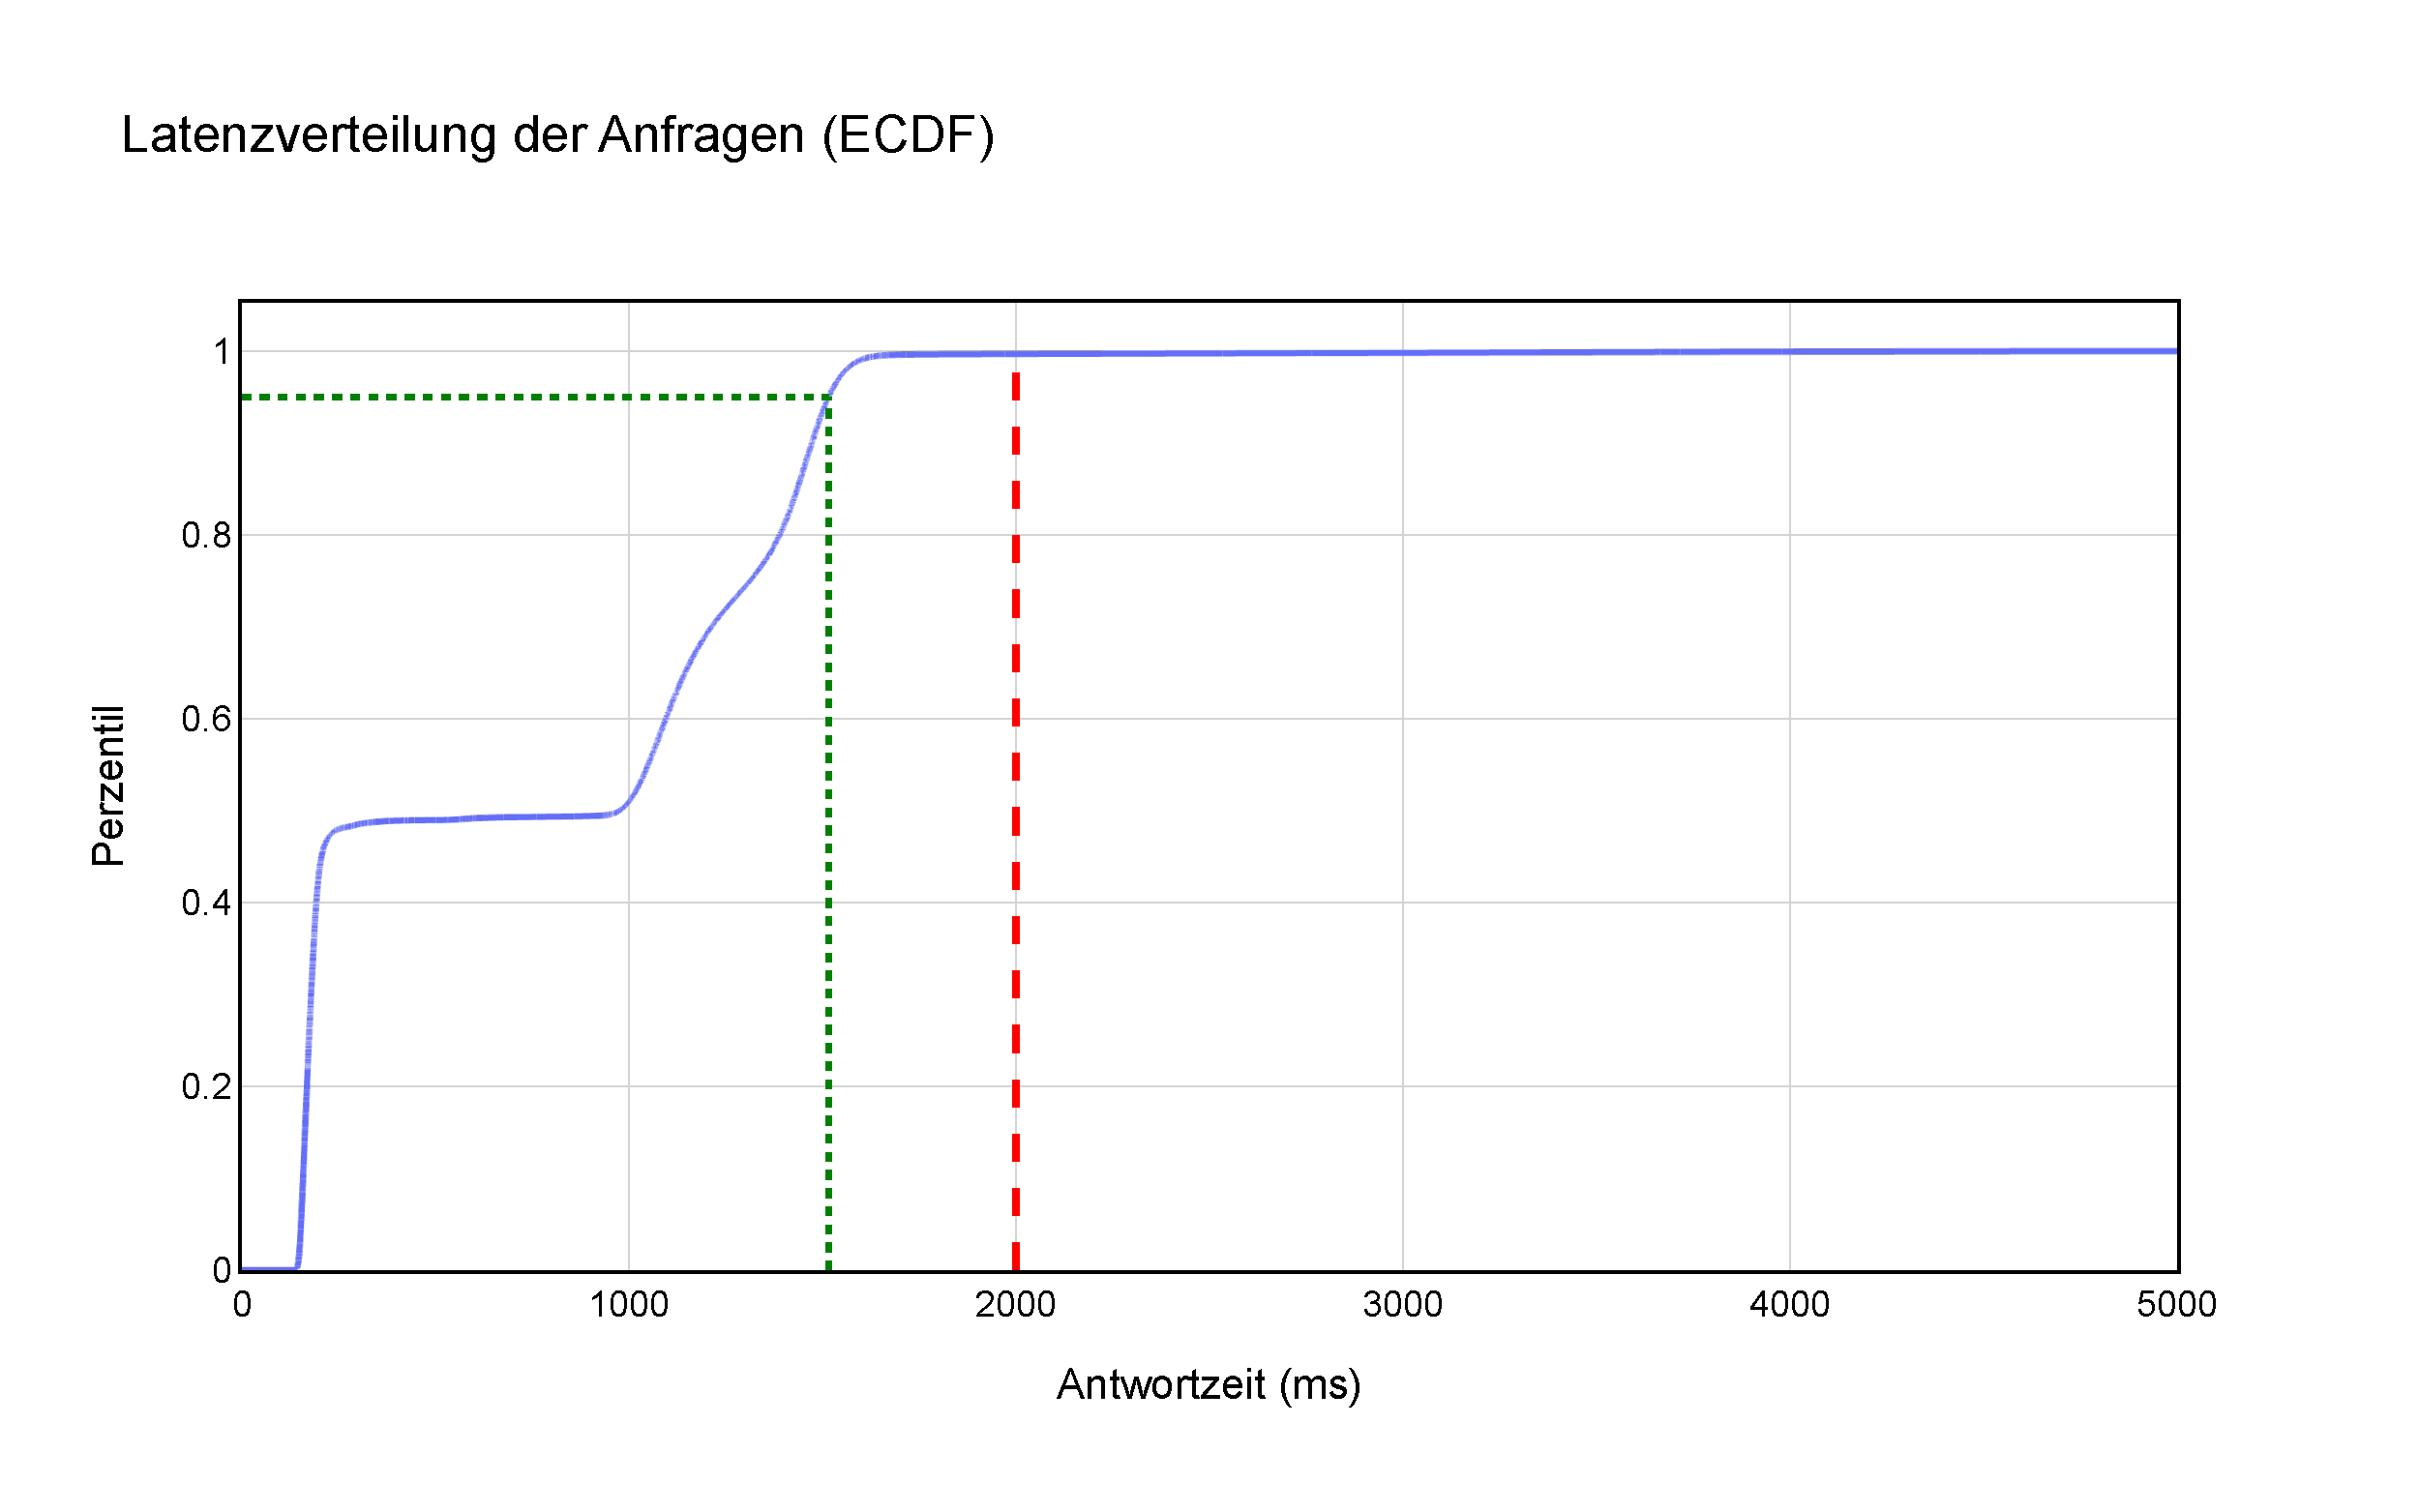
\includegraphics[width=0.8\textwidth]{content/figures/svg/latenzanalyse.pdf}
    \caption{ECDF-Plot der Latenzverteilung. Die rote, gestrichelte Linie markiert das SLO-Ziel von 2000 ms, während die grüne, gepunktete Linie das tatsächlich erreichte 95. Perzentil bei 1562.28 ms zeigt.}
    \label{fig:latenz_ecdf}
\end{figure}


Obwohl es sich um einen Prototyp handelt, wurden weitere, für einen späteren Produktivbetrieb relevante Anforderungen berücksichtigt: Datenschutz und Sicherheit gemäß \ac{DSGVO}, hohe Verfügbarkeit und Ausfallsicherheit sowie Transparenz der Empfehlungslogik zur Stärkung des Nutzervertrauens. Diese Aspekte sind im Entwurf konzeptionell verankert.

\subsection{Rahmenbedingungen}
Die bestehende, auf der \ac{GCP} basierende IT-Infrastruktur der SV-Gruppe setzt die zentralen Rahmenbedingungen. Der Artikelkorpus sowie die aus \ac{GA4} stammenden Nutzerinteraktionsdaten liegen in BigQuery-Tabellen vor. Eine zentrale Ressource bilden hochdimensionale Artikel-Embeddings (3072D), die aus Titeln und Volltexten erzeugt wurden und sich in verwandten Anwendungsfällen (z.\,B. semantische Anzeigenausspielung) bewährt haben. Diese Embeddings werden in dieser Arbeit für den Content-basierten Ansatz wiederverwendet.

Die \texttt{user\_pseudo\_id} ist ein pseudonymer Geräte-/Browser-Identifier. Sie bleibt auf demselben Gerät/Browser meist über mehrere Sitzungen stabil, kann sich jedoch durch Cookie-/App-Resets oder Geräte-/Browserwechsel ändern. Eine Person kann daher mehrere \texttt{user\_pseudo\_id}s haben; umgekehrt kann eine \texttt{user\_pseudo\_id} bei geteilten Geräten mehrere Personen abbilden. Sie ist folglich kein eindeutiger Nutzer, sondern wird hier als Proxy für eine Geräte-/Browser-Instanz genutzt; ein loginbasierter \texttt{user\_id}-Schlüssel lag nicht vor.

Trotz fehlender Eindeutigkeit auf Personenebene ist die user\_pseudo\_id für Empfehlungen praxistauglich, weil (i) ein großer Teil des Traffics anonym ist und ohne Login-ID sonst keinerlei Personalisierung möglich wäre, (ii) sie auf demselben Gerät/Browser über mehrere Sitzungen hinreichend stabil ist, um kurz- bis mittelfristige Präferenzen zu lernen, und (iii) im Nachrichtenkontext vor allem jüngste Interaktionen und der unmittelbare Artikelkontext prädiktiv sind. Letzteres wird durch die Hybridisierung genutzt: Der CBF-Anteil arbeitet kontextuell (wenig abhängig von langlebiger Nutzerhistorie), während der NCF-Anteil gerätebezogene Wiederholungsmuster erfasst. Die Pseudonymität senkt zudem Integrationsaufwand und Datenschutzrisiko gegenüber geräteübergreifendem Identity-Matching. Empirisch zeigt die Offline-Evaluation (vgl. Kapitel~4), dass sich trotz Identitätsfragmentierung robuste Qualitätsgewinne erzielen lassen; die Architektur erlaubt später jederzeit den Wechsel auf eine loginbasierte user\_id.

\begin{figure}[htbp]
    \centering
    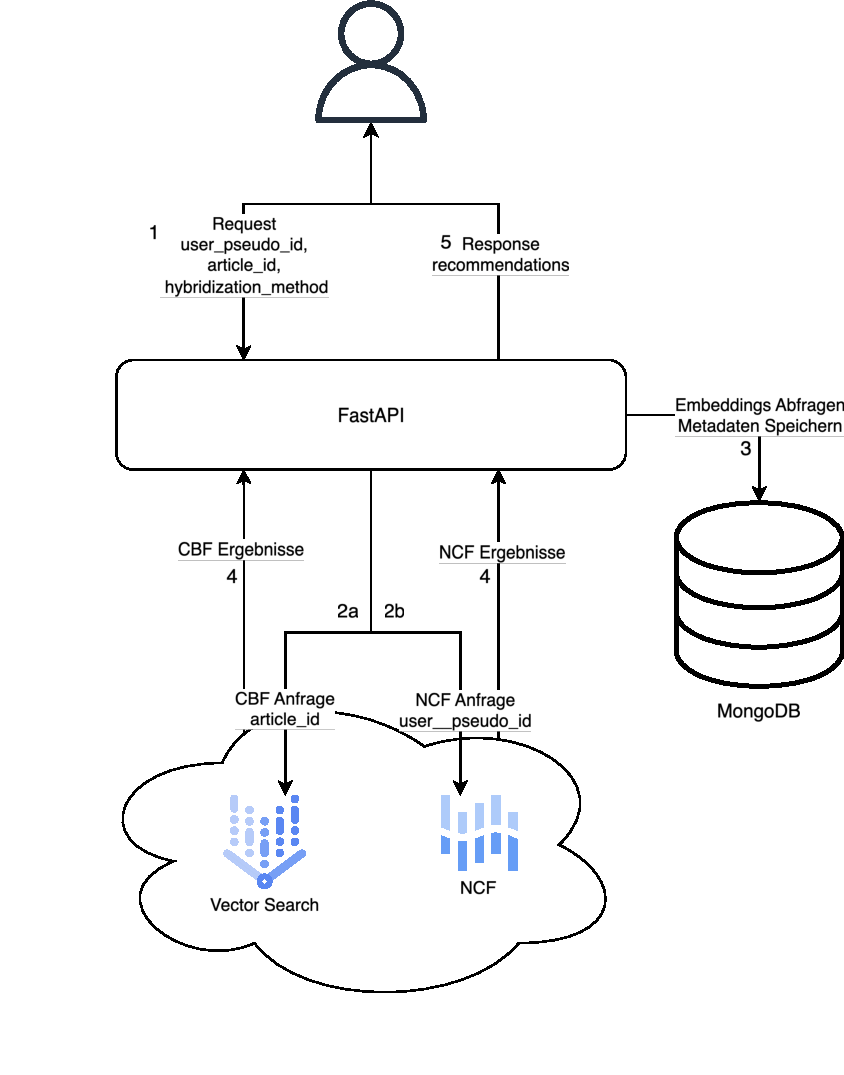
\includegraphics[width=0.6\textwidth]{content/figures/svg/architektur.pdf}
    \caption{Die technologische Architektur des hybriden Empfehlungssystems. Der nummerierte Datenfluss zeigt den Weg einer Anfrage vom Nutzer (1), 
    über die parallelen Abfragen an die ML-Dienste (2a, 2b) und die Datenbank (3), die eintreffenden Ergebnisse (4) bis zur finalen Empfehlung (5).}
    \label{fig:architektur}
\end{figure}
Die technologische Architektur folgt einem cloud-nativen Microservice-Ansatz auf der \ac{GCP}, um die in Abschnitt~\ref{sec:nfr} skizzierten Anforderungen an Skalierbarkeit und Latenz zu erfüllen. Als zentraler Orchestrator dient ein in Python implementierter Service auf Basis von FastAPI. Der Service nimmt Anfragen entgegen, steuert die Modell-Endpunkte, aggregiert die Teilergebnisse und führt die Hybridisierung aus. Das Design ist modular, um künftig alternative Hybridisierungsstrategien mit geringem Integrationsaufwand aufnehmen zu können. Für die latenzkritische Online-Auslieferung werden der Artikelkorpus und Embeddings in einer operativen Datenbank vorgehalten; die ML-Modelle sind auf Vertex~AI deployt. Während des Deployments auf Vertex~AI aufgetretene Out-of-Memory-Probleme konnten durch angepasste Konfiguration (u.\,a. Begrenzung der Worker-Prozesse) behoben werden.

\label{sec:api_design}
Das Herzstück des Systems bildet der API-Service, der die externe Schnittstelle und die interne Orchestrierung bereitstellt. Die API exponiert einen REST-Endpunkt unter \texttt{/v1/recommendations} mit einem JSON-basierten Datenvertrag. Eine Anfrage umfasst die \texttt{user\_pseudo\_id}, die \texttt{article\_id} als Kontext sowie die gewünschte Hybridisierungsstrategie. Die Implementierung nutzt die asynchrone Leistungsfähigkeit von FastAPI (\ac{ASGI}) und orchestriert pro Anfrage parallele Aufrufe der untergeordneten ML-Dienste und der Datenbank. Nach dem Zusammenführen der Teilergebnisse wird die Hybridisierungslogik angewandt und die finale Empfehlungsliste zurückgegeben. Eingebaute Schema-Validierung und die automatische Generierung einer interaktiven API-Dokumentation unterstützen eine robuste Integration.

\label{sec:cbf_service}
Der \ac{CBF}-Ansatz wird mittels Vertex~AI Vektorsuche realisiert. Das Auffinden thematisch ähnlicher Artikel zu einem gegebenen Beitrag entspricht einer Nearest-Neighbor-Suche in einem hochdimensionalen Vektorraum. Eine exakte Brute-Force-Suche ist für Echtzeitanforderungen nicht praktikabel; daher kommt ein \ac{ANN}-Verfahren zum Einsatz. Vertex~AI basiert hierbei auf Googles \ac{ScaNN}, das zwei Prinzipien kombiniert:
\begin{itemize}
    \item \textbf{Partitionierung des Vektorraums:} Der Index unterteilt den Raum in viele Partitionen. Bei einer Anfrage werden nur die wahrscheinlichsten Partitionen durchsucht, wodurch der Suchraum drastisch reduziert wird.
    \item \textbf{Vektorquantisierung:} Innerhalb der Partitionen werden Vektoren komprimiert repräsentiert, um Speicherbedarf und Distanzberechnungen zu optimieren. Google nutzt hierfür u.\,a. anisotrope Vektorquantisierung, um Informationsverluste zu minimieren \cite{avq_2020}.
\end{itemize}
ScaNN identifiziert effizient die vielversprechendsten Partitionen und berechnet dort Distanzen auf den quantisierten Vektoren. Die fortlaufende Optimierung solcher Indexierungsstrategien wird durch Arbeiten wie SOAR, einen Nachfolger-Ansatz zur Verbesserung der Indexeffizienz, dokumentiert \cite{soar_2023}. Der zugrunde liegende Trade-off ist eine minimale Einbuße an Genauigkeit zugunsten deutlicher Gewinne bei der Abfragegeschwindigkeit.

\label{sec:ncf_service}
Als kollaborativer Filteransatz wird ein \ac{NCF}-Modell eingesetzt. Klassische \ac{MF}-Methoden modellieren Nutzer–Artikel-Interaktionen als Skalarprodukt latenter Vektoren und sind damit in ihrer Ausdrucksstärke auf lineare Zusammenhänge beschränkt. Das NCF-Framework ersetzt dieses Skalarprodukt durch eine neuronale Architektur; konkret approximiert ein \ac{MLP} eine nichtlineare Interaktionsfunktion direkt aus den Daten \cite{he_neural_2017}. Dadurch kann das Modell komplexe Muster im Interaktionsverhalten erfassen und personalisierte Empfehlungen generieren. Für den Echtzeitbetrieb wird das trainierte Modell auf einem dedizierten Vertex~AI-Endpoint bereitgestellt. In der vorliegenden Anwendung wird der im NCF beobachtete Popularity Bias im Rahmen der Hybridisierung gezielt genutzt, um die Filterblase des CBF-Anteils aufzubrechen und Diversität zu erhöhen (vgl. Kapitel~4).

\subsection{Datenbasis und Einschränkungen}
\label{sec:data}
Der Datensatz \textit{SM-News-Jan25} umfasst ausschließlich \ac{GA4}-Interaktionsdaten aus dem Januar 2025. Aus Kostengründen wird das NCF-Modell auf den ersten drei Wochen trainiert und in der vierten Woche getestet. Eine zentrale Eigenschaft ist die stark rechtsverschobene Verteilung sowohl der Artikelpopularität als auch der Nutzeraktivität (Long-Tail-Verteilung), ein für Mediendaten typisches Muster und eine Kernherausforderung für Empfehlungssysteme \cite{wu_personalized_2022, raza_news_2020}.
% content/figures/plot_artikelverteilung_train.tex

\begin{figure}[H]
    \centering
    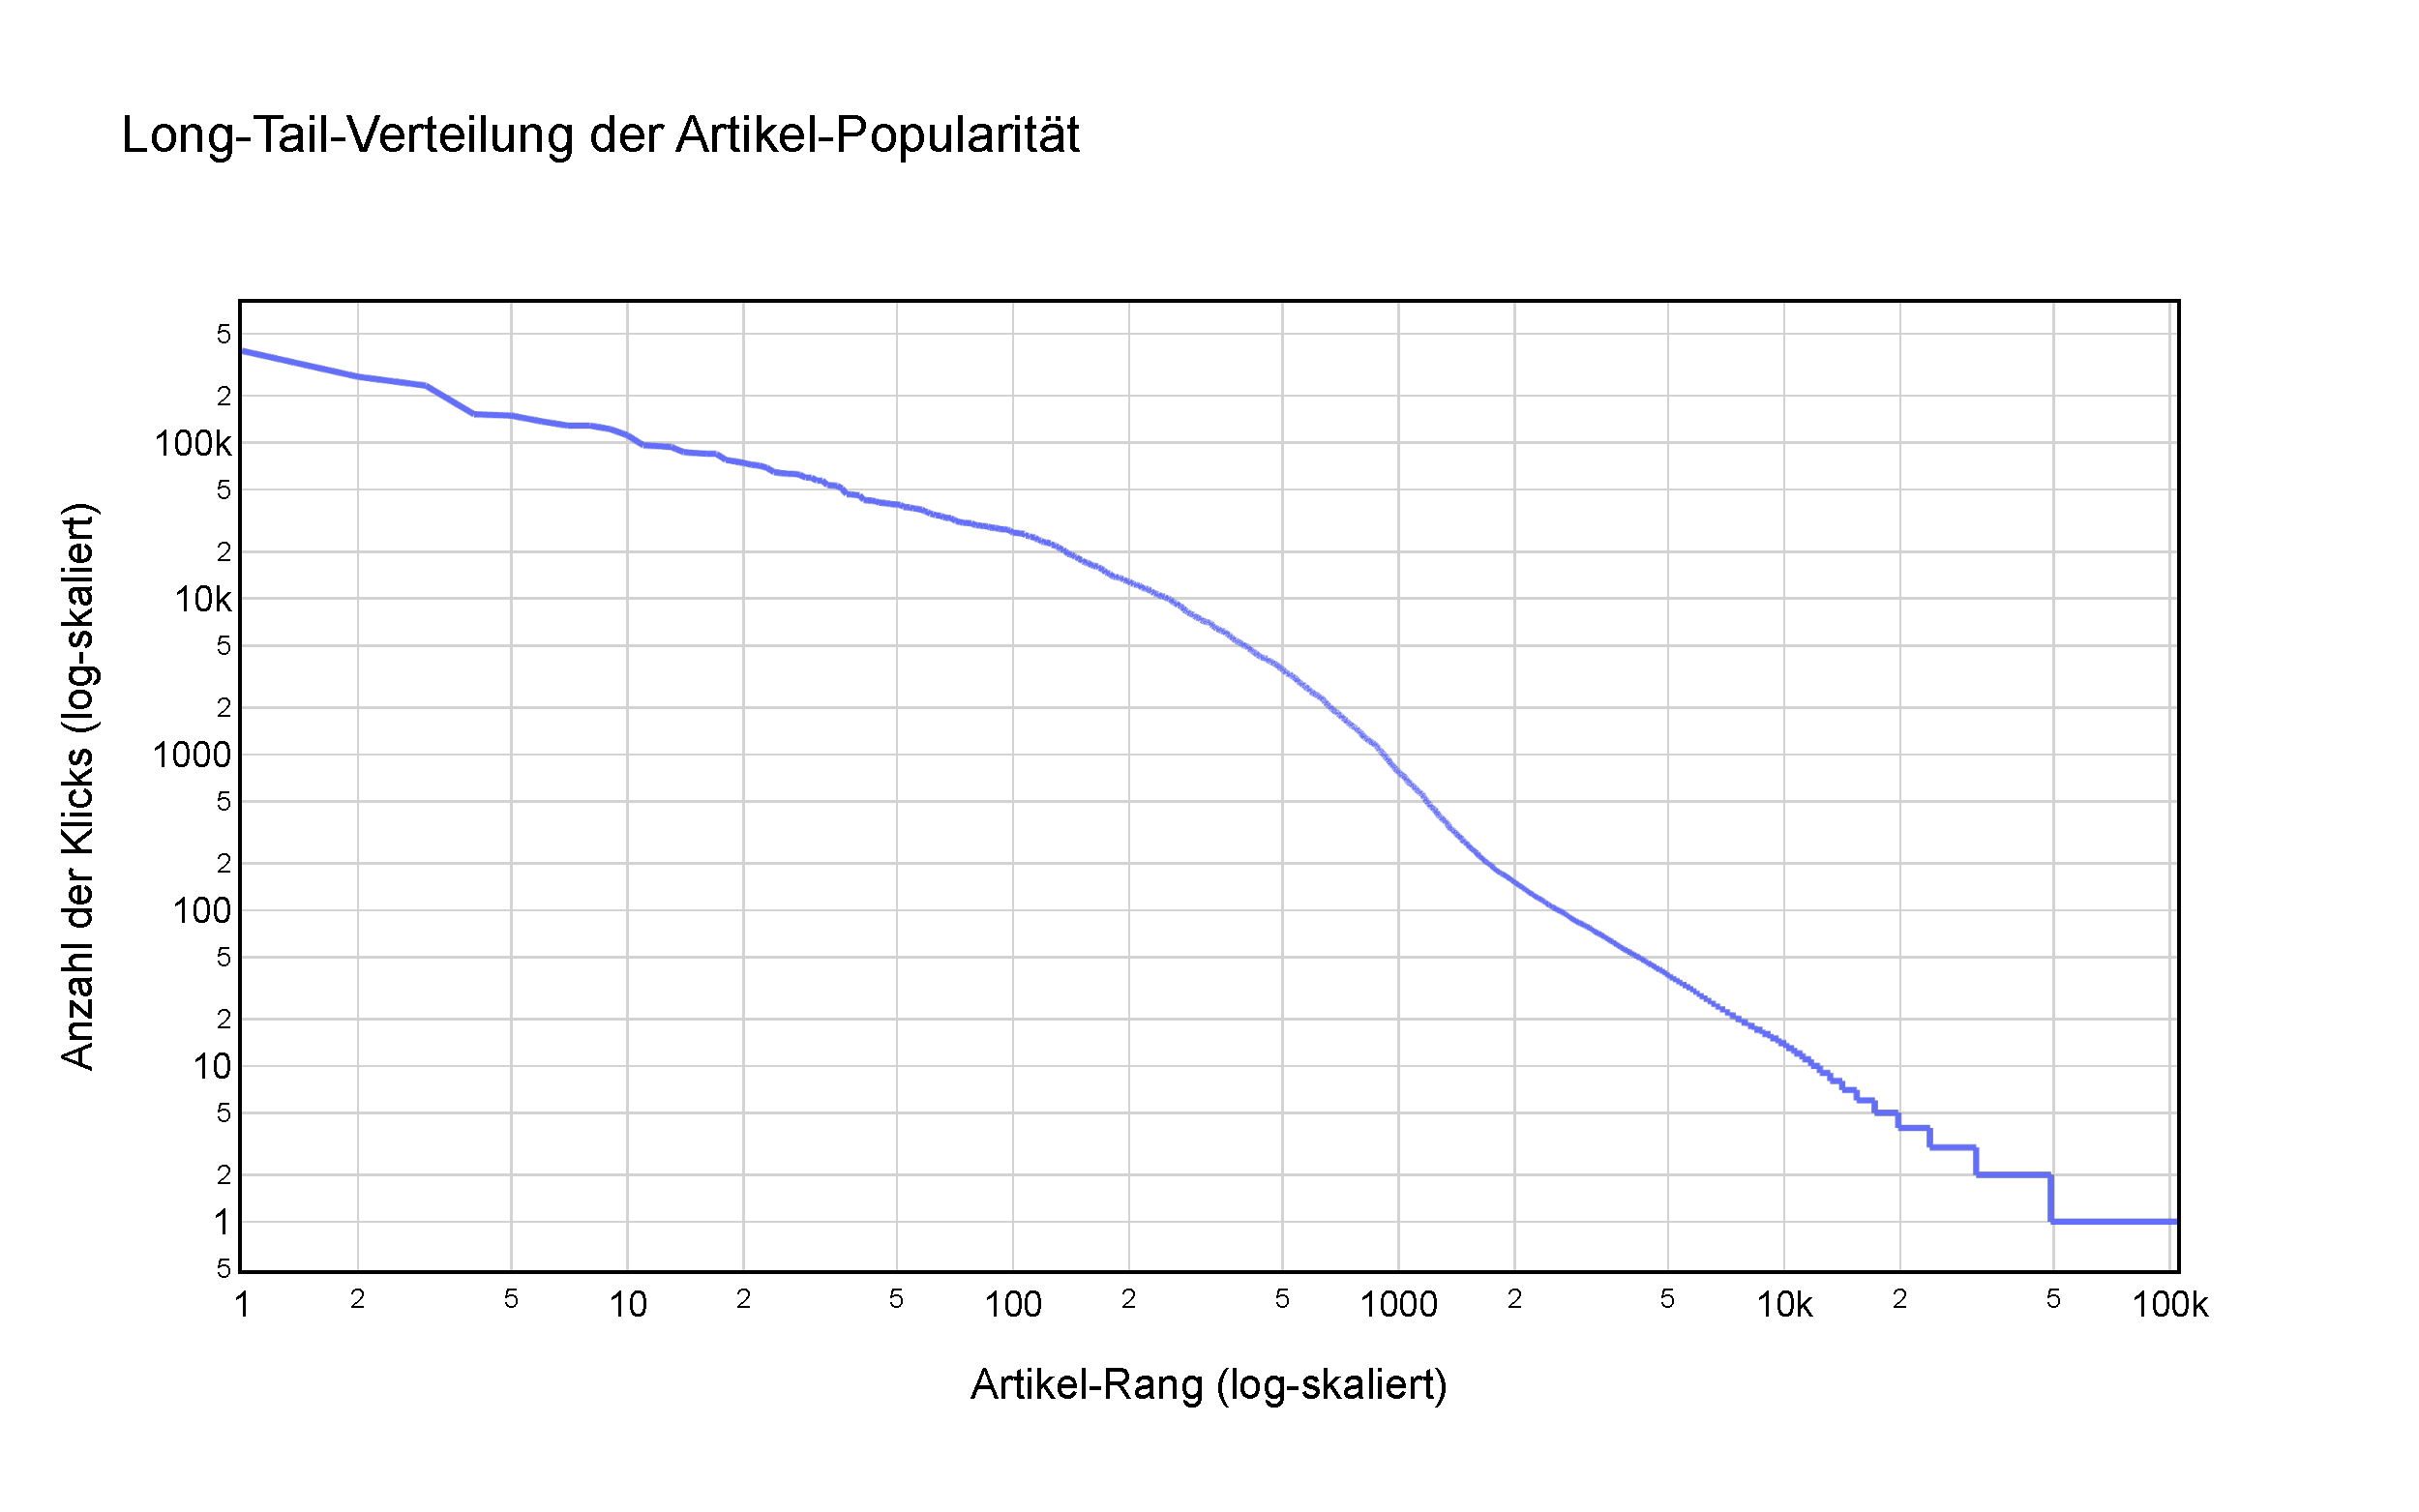
\includegraphics[width=0.9\textwidth]{content/figures/svg/artikel_verteilung_train.pdf}
    \caption{Popularitätsverteilung der Artikel im Trainingsdatensatz. Die Grafik zeigt, dass eine geringe Anzahl von Artikeln einen Großteil der Klicks auf sich vereint, während die Mehrheit der Artikel nur wenige Interaktionen erhält (Long-Tail).}
    \label{fig:artikelverteilung_train}
\end{figure}

Die Long-Tail-Struktur manifestiert sich in zwei Dimensionen:
\begin{itemize}
    \item \textbf{Artikelpopularität:} Wie in Abbildung~\ref{fig:artikelverteilung_train} ersichtlich, konzentriert sich ein \newline überproportional großer Anteil der Seitenaufrufe auf wenige virale „Hit“-Artikel (Kopf der Verteilung). Die kurze Lebensdauer von Nachrichtenartikeln verstärkt diesen Effekt zusätzlich.
    \item \textbf{Nutzeraktivität:} Analog zeigt sich beim Nutzerverhalten eine kleine Kohorte hochaktiver „Power-Nutzer“, die einen Großteil der Klicks generiert, während die Mehrheit nur sporadisch interagiert.
\end{itemize}
Diese ungleiche Verteilung induziert einen inhärenten Popularity Bias: Naive Modelle empfehlen tendenziell wiederholt dieselben Bestseller-Artikel, was Personalisierung untergräbt und das Risiko einer Filterblase erhöht. Gleichzeitig entsteht ein Kaltstart-Problem für Nischeninhalte im Long Tail. Eine zentrale Zielsetzung dieser Arbeit ist folglich die Konzeption eines Systems, das den Popularity Bias aktiv ausbalanciert und relevante Nischeninhalte an passende Nutzer ausspielt.
% content/figures/plot_nutzerverteilung_train.tex

\begin{figure}[H]
    \centering
    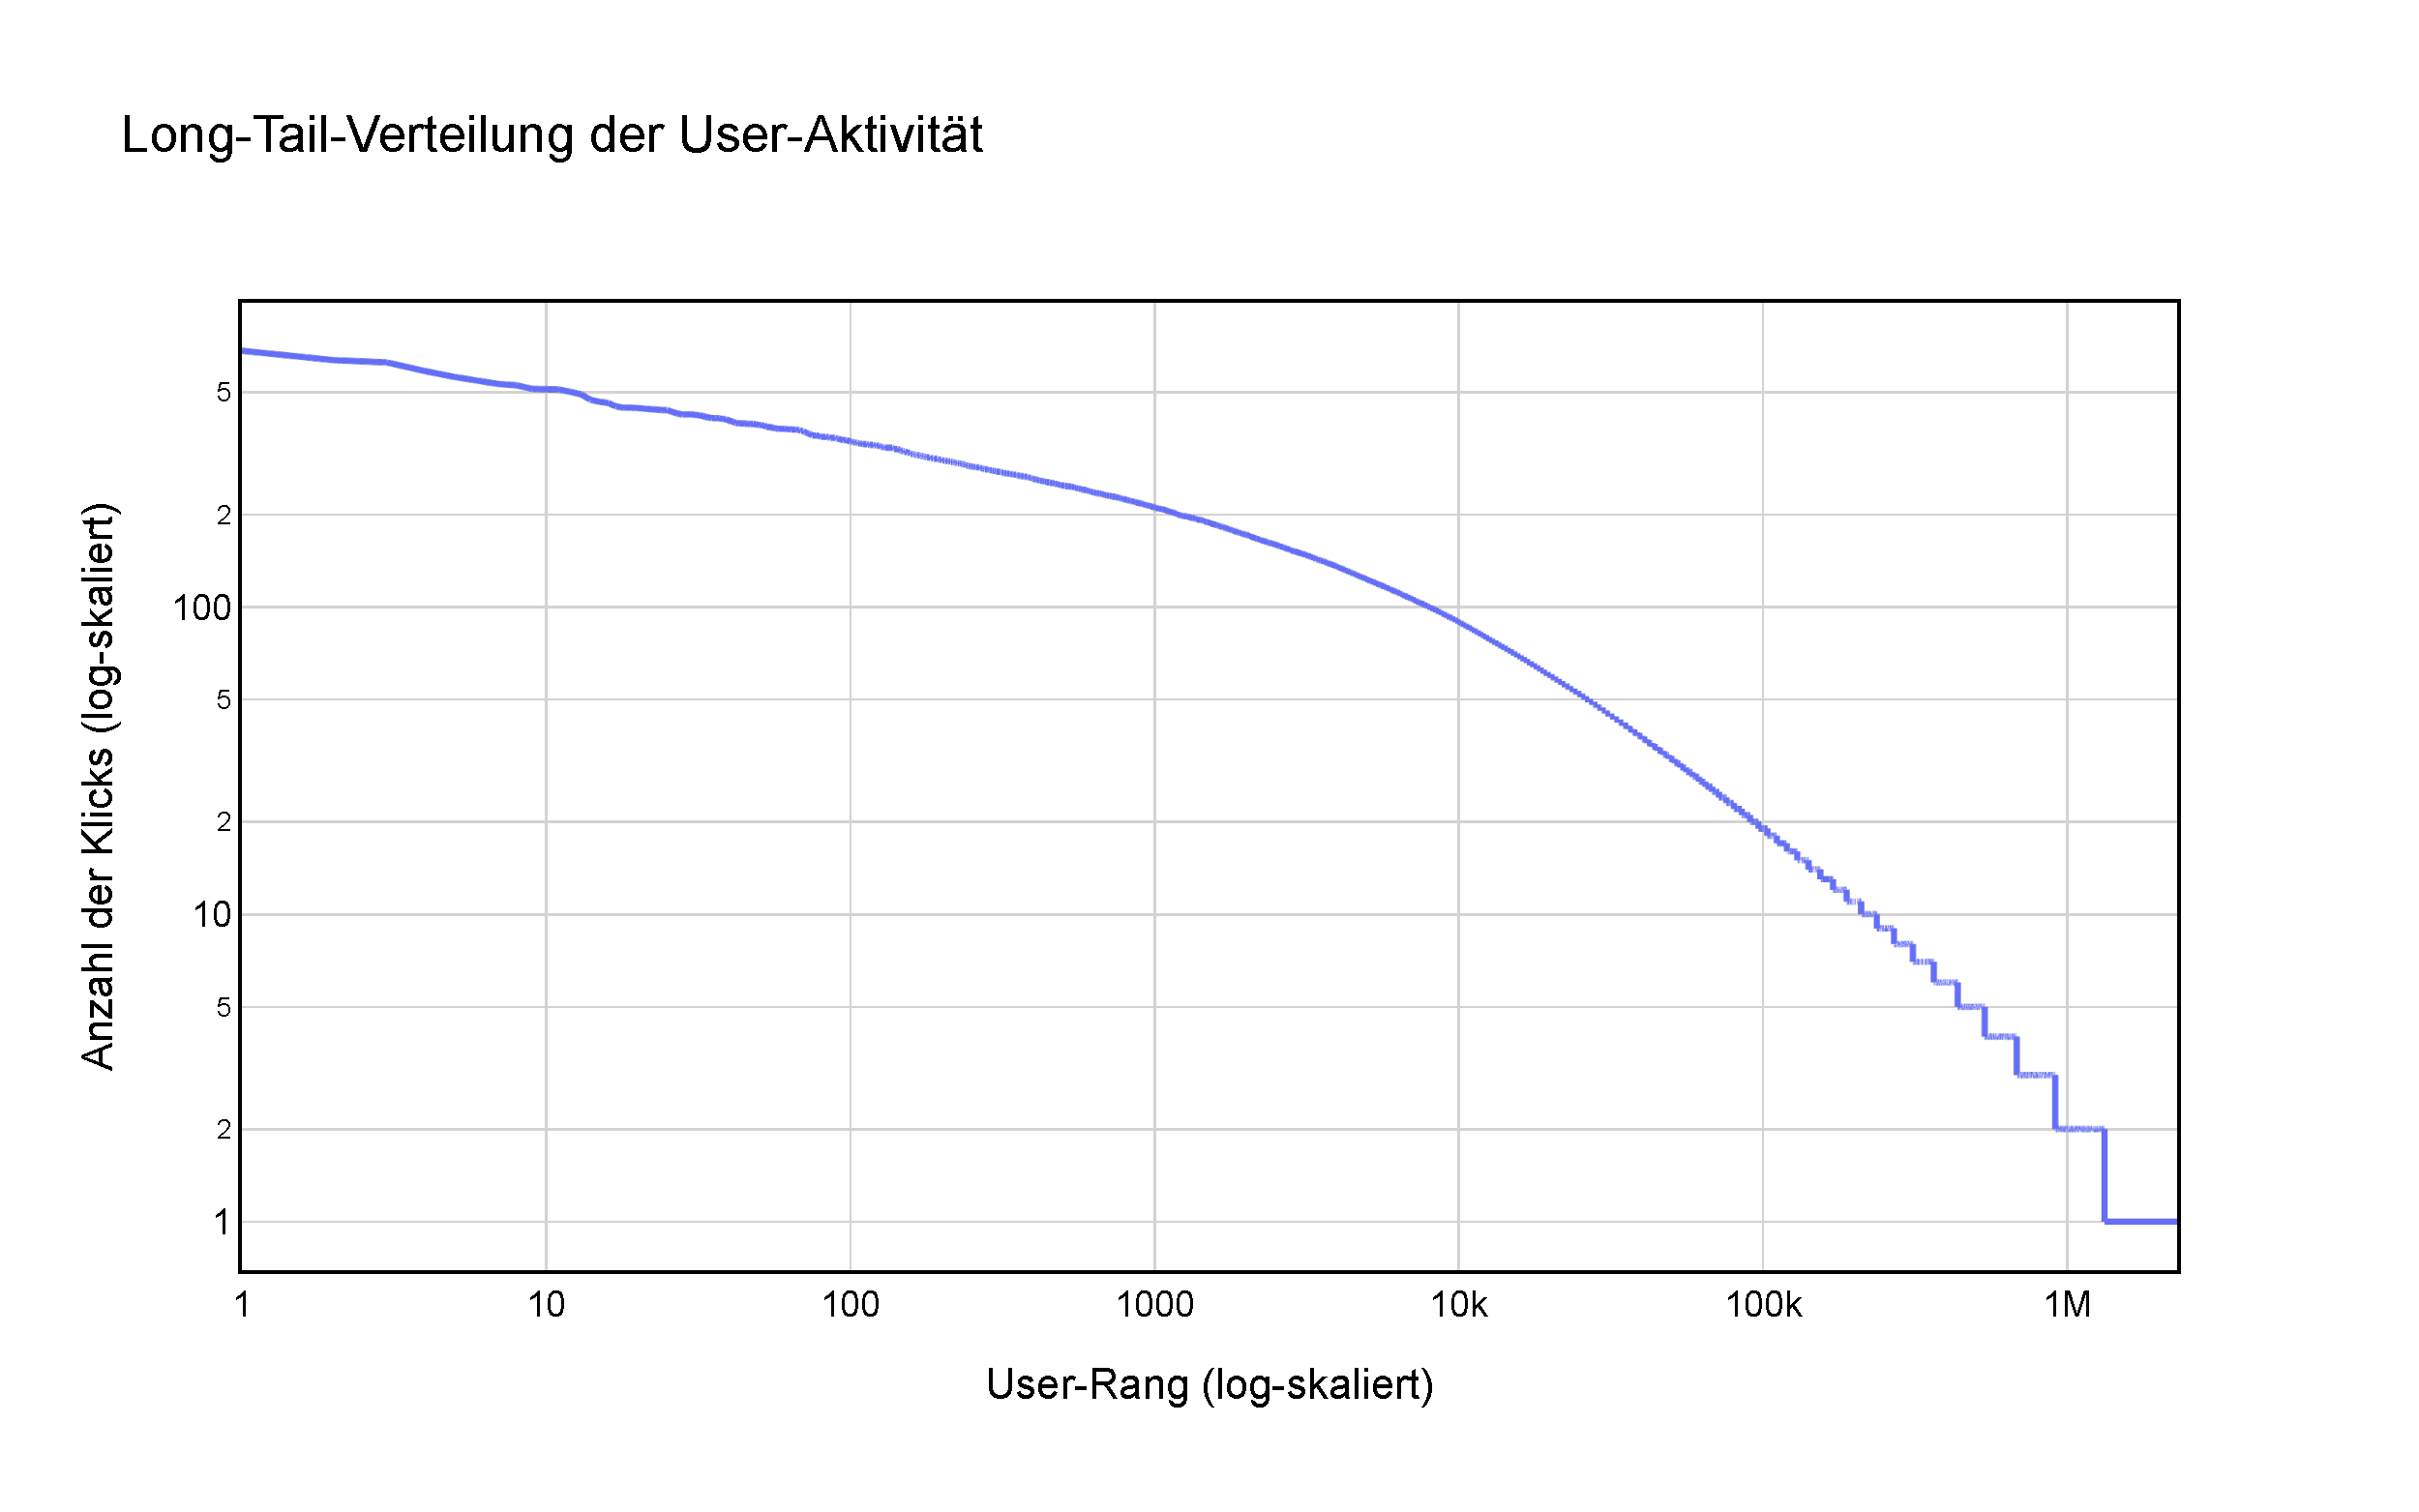
\includegraphics[width=0.9\textwidth]{content/figures/svg/nutzer_verteilung_train.pdf}
    \caption{Verteilung der Nutzeraktivität im Trainingsdatensatz. Die Darstellung verdeutlicht die typische Long-Tail-Verteilung: Eine große Anzahl von Nutzern interagiert nur selten mit Artikeln, während eine kleine Gruppe von "Power-Nutzern" für einen Großteil der Klicks verantwortlich ist.}
    \label{fig:nutzerverteilung_train}
\end{figure}

Die statistischen Kennzahlen des Trainingsdatensatzes sind in Tabelle~\ref{tab:train_stats} zusammengefasst.
% content/tables/statistiken_trainingsdaten.tex

\begin{table}[H]
    \centering
    \caption{Statistische Kennzahlen des Trainingsdatensatzes, basierend auf den Klick-Logs der ersten drei Januarwochen.}
    \label{tab:statistiken_training}
    \begin{tabular}{lr}
        \toprule
        \textbf{Metrik} & \textbf{Wert} \\
        \midrule
        Gesamte Interaktionen (Klicks) & 11.412.116 \\
        Einzigartige user\_pseudo\_ids & 2.294.733 \\
        Einzigartige Artikel & 104.462 \\
        \bottomrule
    \end{tabular}
\end{table}
\label{tab:train_stats}

Zur Nutzung der Klick-Events im \ac{NCF}-Modell werden diese in eine \newline User–Item-Interaktionsmatrix überführt. Zeilen repräsentieren eindeutige Nutzer, Spalten eindeutige Artikel des Trainingszeitraums. Eine Zelle $(i,j)$ erhält den Wert 1, wenn Nutzer $i$ mit Artikel $j$ interagiert hat, andernfalls 0. Die resultierende binäre Matrix mit circa 2{,}3~Mio.\ Nutzern und 104{,}000 Artikeln weist eine Dichte von unter 0{,}005\,\% auf und ist damit extrem dünn besetzt. Diese Sparsity ist für \ac{CF}-Modelle herausfordernd, da je Nutzer nur wenige Interaktionen im Verhältnis zur Gesamtheit der Artikel vorliegen und Generalisierung auf neue User–Item-Paare erschwert wird.

Bei der Interpretation der Ergebnisse sind folgende Limitationen zu berücksichtigen:
\begin{itemize}
    \item \textbf{Zeitlicher Rahmen:} Der Datensatz deckt ausschließlich den Januar 2025 ab und bildet damit eine Momentaufnahme. Saisonale Effekte (z.\,B. Feiertage) oder längerfristige Trends können nicht erfasst werden.
    \item \textbf{Implizites Feedback:} Als Signal dienen ausschließlich Klicks. Dieses implizite Feedback ist zwar reichhaltig, jedoch mehrdeutig: Ein Klick ist kein direkter Indikator für Zufriedenheit (z.\,B. bei sofortigem Absprung). Weitere Signale wie Verweildauer werden im Prototyp nicht berücksichtigt.
    \item \textbf{Offline-Evaluation:} Die Modellgüte wird offline auf historischen Daten anhand etablierter Metriken (z.\,B. \ac{nDCG}) evaluiert. Die tatsächliche Wirkung auf Nutzerverhalten im Live-Betrieb lässt sich damit nur approximieren. Ein Online-A/B-Test wäre der nächste Schritt, um den Business Impact auf KPIs wie Sitzungsdauer oder Nutzerbindung zu messen.
\end{itemize}